\section{索引节点层}

我们使用ls -l时除了看到文件名,还看到了文件元数据
\begin{lstlisting}[]
[root@localhost linux]# ls -l
总用量 12
-rwxr-xr-x. 1 root root 7438 "9月 13 14:56" a.out
-rw-r--r--. 1 root root 654  "9月 13 14:56" test.c
\end{lstlisting}

为了能解释清楚inode我们先简单了解一下Linux的文件系统
\begin{figure}[H]
    \centering
    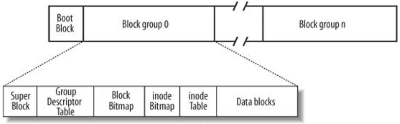
\includegraphics{figures/07-04-磁盘.png}
    \caption{磁盘文件系统图}
\end{figure}

Linux ext2文件系统,上图为磁盘文件系统图(内核内存映像肯定有所不同),磁盘是典型的块设备,硬盘分区被划分为一个个的block。一个block的大小是由格式化的时候确定的,并且不可以更改。

一个block在磁盘上的布局如下:
\begin{figure}[H]
    \centering
    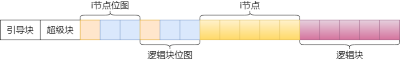
\includegraphics{figures/07-04-inode.png}
    \caption{block布局}
\end{figure}
由上图可知,文件系统的开头通常是由一个磁盘扇区所组成的引导块,该部分的主要目的是用于对操作系统的引导。一般只在启动操作系统时使用。
随后是超级块,超级块主要存放了该物理磁盘中文件系统结构的相关信息,并且对各个部分的大小进行说明。
inode块位图,data块位图记录了在inode块和data块中哪些块已被使用,以便找到空闲的位置
inode块和data块则是实际存放inode和数据的地方,data存放文件的内容,inode存放文件元数据并指向所属的data的地址

Linux为了对超级块,inode块,数据块这三部分进行高效的管理,Linux创建了几种不同的数据结构,分别是文件系统类型、inode、dentry等几种。
超级块反映了文件系统整体的控制信息。
dentry是反映出某个文件系统对象在全局文件系统树中的位置。
inode则反映了文件系统对象中的一般元数据信息。

\textbf{我们可以得出一个结论:inode存放了文件元数据信息,并指向文件的内容}
所以上文的`ls -l`实际上就是使用了inode的文件元数据
而npucore中虽然使用了fat32文件系统,但在代码层面上同样引入了inode这个概念,服务于文件相关系统调用的索引节点层的代码在 `vfs.rs` 中。

简单文件系统层实现了磁盘布局并能够将磁盘块有效的管理起来。但是对于文件系统的使用者而言,他们往往不关心磁盘布局是如何实现的,而是更希望能够直接看到目录树结构中逻辑上的文件和目录。为此需要设计索引节点 `Inode` ,它屏蔽了简单文件系统层对磁盘的操作,让文件系统的使用者能够直接对文件和目录进行操作。
\begin{lstlisting}[language={Rust}, label={code:inode},
	caption={easy-fs/src/fs/fat32/vfs.rs}]
pub struct Inode {
    /// Inode lock: for normal operation
    inode_lock: RwLock<InodeLock>,
    /// File Content
    file_content: RwLock<FileContent>,
    /// File cache manager corresponding to this inode.
    file_cache_mgr: PageCacheManager,
    /// File type
    file_type: Mutex<DiskInodeType>,
    /// The parent directory of this inode
    parent_dir: Mutex<Option<(Arc<Self>, u32)>>,
    /// file system
    fs: Arc<EasyFileSystem>,
    /// Struct to hold time related information
    time: Mutex<InodeTime>,
    /// Info Inode to delete file content
    deleted: Mutex<bool>,
}
\end{lstlisting}

inode\_lock: 该inode的读写锁
file\_content:指向文件的内容
file\_cache\_mgr:指向管理该inode的PageCacheManager
file\_type:文件类型
parent\_dir:指向父目录的inode以及该inode在父目录的位置
fs:指向该inode所属的简单文件系统
time:该文件的相关时间属性
delete:一个标识,控制在该inode执行析构函数时是否释放文件内容的区域

利用这个inode结构体,文件系统的使用者就可以对文件系统进行一些常用操作:
\begin{lstlisting}[language={Rust},
	caption={easy-fs/src/fs/fat32/vfs.rs}]
// 创建目录项
fn create_dir_ent(
    &self,
    inode_lock: &RwLockWriteGuard<InodeLock>,
    short_ent: FATShortDirEnt,
    long_ents: Vec<FATLongDirEnt>,
) -> Result<u32, ()>

// 删除目录项
fn delete_dir_ent(
    &self,
    inode_lock: &RwLockWriteGuard<InodeLock>,
    offset: u32,
) -> Result<(), ()>

// 创建硬链接(link)
impl Inode {
pub fn link_par_lock(
    &self,
    inode_lock: &RwLockWriteGuard<InodeLock>,
    parent_dir: &Arc<Self>,
    parent_inode_lock: &RwLockWriteGuard<InodeLock>,
    name: String,
) -> Result<(), ()>

// 删除硬链接(unlink)
pub fn unlink_lock(
    &self,
    _inode_lock: &RwLockWriteGuard<InodeLock>,
    delete: bool,
) -> Result<(), isize>
    
// ls
pub fn ls_lock(
    &self,
    inode_lock: &RwLockWriteGuard<InodeLock>,
) -> Result<Vec<(String, FATShortDirEnt)>, ()>
  
// 获取文件时间相关信息
pub fn time(&self) -> MutexGuard<InodeTime>
    
// ...
\end{lstlisting}